\section{Ahuthentication Service}



\indent
\indent
This service provides user authentication. It is composed of three components: the hash service, the database, and the main service (Figure \ref{auth:xxdfdfdfdf}).

The password is store securely, is hashed and salted using the hash service and then the hash and salt is stored in the database.

The database is replicated using the master follower topology. Create, update, and delete operations are always performed in the master, read operations are performed in followers. 

\begin{figure}[H]
\begin{center}
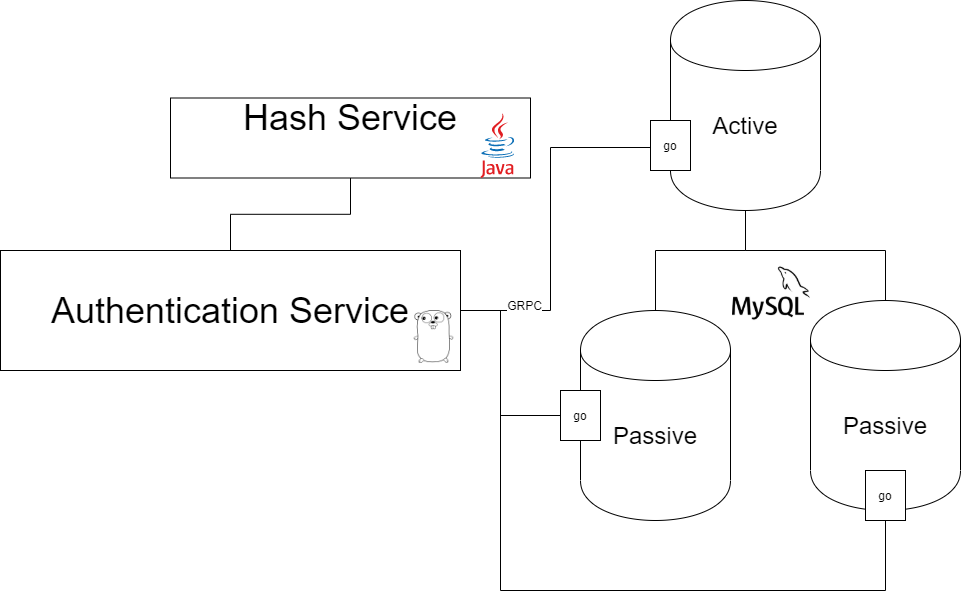
\includegraphics[width=120mm,scale=1]{img/auth/auth-main-uml.png}
\caption{Authentication Service- UML.}
\label{auth:xxdfdfdfdf}
\end{center}

\end{figure}


\subsection{Database Replication}

\indent
\indent
Replication it has been set up using MySQL 5.7 (See Appendix \ref{appendix:SetupReplication}),  we have set up a master and a replicate running in different Virtual Machine using Azure services. Using the instruction in Appendix \ref{appendix:SetupReplication} is possible to add more followers, for do tables in master need to be locked for a few minutes.

The load balancing is done using Round Robin, and standards go grpc librarie. helps in performance because the most used operation is to get user data or token to check authentication.

Is implemented as client-side replication, the client chooses a server one at the time to make the calls, the client in this situation is the authentication service, and the server is the authentication dba. The load balancing is implemented in the authentication service(Figure \ref{auth:createusersequence}).

\begin{figure}[h]
	\begin{center}
		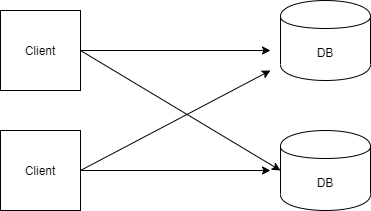
\includegraphics[width=90mm,scale=1]{img/auth/client-side-load-balancer.png}
		\caption{Authentication Service- Create User Sequence Diagram.}
		\label{auth:loadbalancerdiagram}
	\end{center}
\end{figure}

\subsection{Endpoints} 

\subsubsection{Create User}

\indent
\indent
Users create an account, and when this happens, a new entry is created in the authentication database. Also, a new entry is created in the profiles database (Figure   \ref{auth:createusersequence}). To create a user, this service needs to communicate with the profiles service.



\begin{figure}
\begin{center}
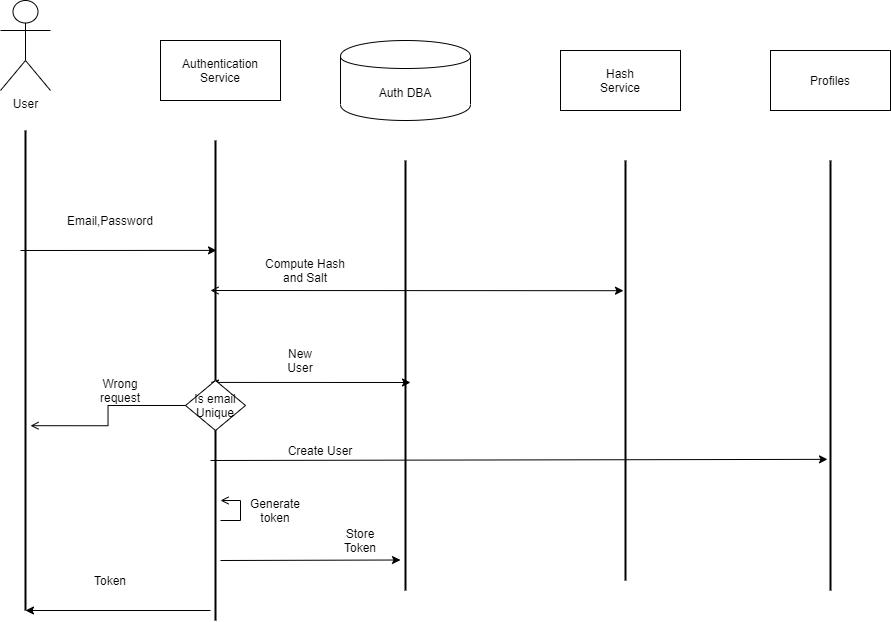
\includegraphics[width=90mm,scale=1]{img/auth/CreateUser_sequence.png}
\caption{Authentication Service- Create User Sequence Diagram.}
\label{auth:createusersequence}
\end{center}
\end{figure}

\subsubsection{Login user}
\indent
\indent
To login a user, we perform the followings steps (Figure \ref{auth:loginsequence}):
\begin{itemize}

\item Get user data from the authentication database.
\item	Check the password using the hash service.
\item	If the password is valid will generate a unique token, it stores the token in the database and sends the response to the client.
\end{itemize}

\begin{figure}
\begin{center}
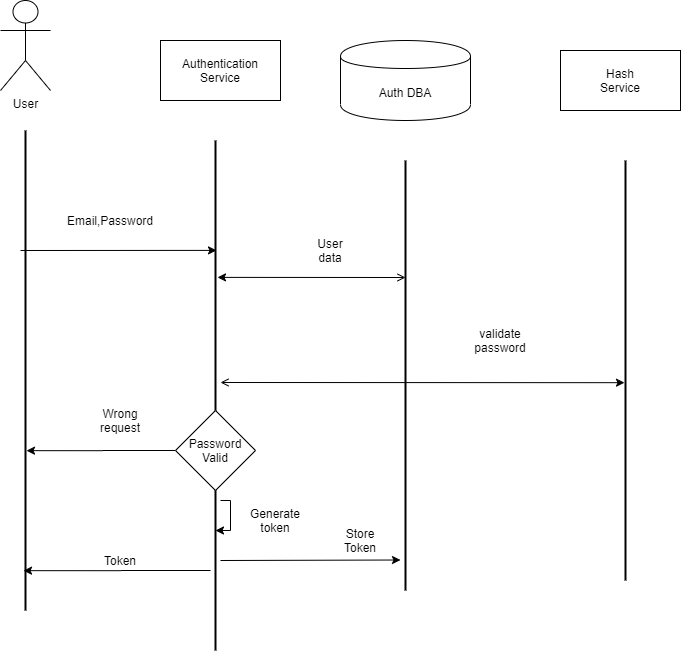
\includegraphics[width=90mm,scale=1]{img/auth/login-sequence.png}
\caption{Authentication Service- Login Sequence Diagram.}
\label{auth:loginsequence}
\end{center}

\end{figure}


\subsubsection{Check Token}

\indent
\indent
The most used endpoint, here is where replication plays a role for fast checking tokens. This is used in the most requests to all services to ensure security across the application (Figure \ref{auth:checktokensequence}).


\begin{figure}
\begin{center}
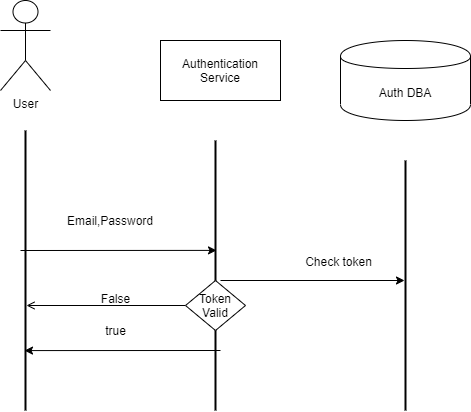
\includegraphics[width=90mm,scale=1]{img/auth/check-token-sequence.png}
\caption{Authentication Service- Check Token Sequence Diagram.}
\label{auth:checktokensequence}
\end{center}
\end{figure}

\subsubsection{Log out}
\indent
\indent
The request includes the token, and that token is removed from the sessions table in the authentication database.


\subsection{Authentication DBA}
\indent
\indent
This program provides access to the authentications database. Is written in go and runs in a docker container, it connects to a MySQL database running in localhost. The application communicates with the main authentication service through a grpc interface.

\subsubsection{The database}


\begin{figure}
\begin{center}
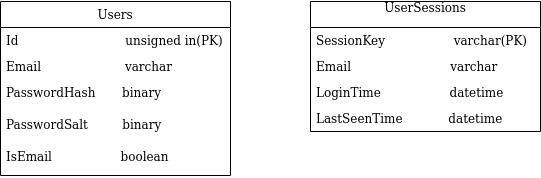
\includegraphics[width=90mm,scale=1]{img/auth/auth-db.png}
\caption{Authentication DBA- Authentication Database.}
\label{auth:authdbuml}
\end{center}

\end{figure}

\indent
\indent
The authentication database store the necessary user data for authentication and login.

 It is composed of two tables: the authentication table and the sessions table. The authentication table contains the user name, the password hash, and the password salt(Figure \ref{auth:authdbuml}).
 
  The user name is the email and is the unique identifier for all the systems, is not the primary key of the database, but is indexed for quick access. For this database, an extra integer field is added as the primary key. The password hash and salt are 32 bytes binaries strings. The sessions table uses a unique session key as a primary key for a quick check if a session exists. 
  
  When a user login a session is created and stored in this table. The user then can log in to the application using that session. When the user logs out, the session is deleted from the database.


\subsubsection{Endpoints}
\begin{itemize}
\item AddUser() : Create a new user in the database. When the user creates the account, it will create the profile automatically in the profiles database.

\item GetUser(): Returns the user data used to authenticate the user.

\item UpdateUser(): Update the user data, is used for changing the password.

\item CreateSeassion(): Create a new session in the database. Used when the user login  using the password.

\item GetSeassion() : Return a user session if exist. Used to check if the session exists so the user can log in without the password.

\item DeleteSession : Delete user session if exits. Used when the user logs out from the device.

\end{itemize}

\subsection{The Hash Service}

\indent
\indent
This service creates a password salted password hash using a randomly generated salt. It has been adapted from a Distributed Systems project from semester 7.
It checks the password in fix amount of time for security reasons. Attackers can guess passwords guess by comparing the time it takes to validate a password.
\newpage